\documentclass[journal]{IEEEtran}

\usepackage{blindtext}
\usepackage{graphicx}
\usepackage{hyperref}
\usepackage{listings}

\usepackage{tikz}
\usetikzlibrary{arrows,shapes,positioning}
\usetikzlibrary{calc,decorations.markings}

\tikzstyle{block} = [
  rectangle, draw, rounded corners, text centered, text width =
  7em, minimum height = 2em
]
\tikzstyle{dottedblock} = [
  rectangle, draw, rounded corners, text centered, text width =
  7em, minimum height = 2em,dashed
]
\tikzstyle{line} = [draw, -latex']

\usepackage[backend=bibtex]{biblatex}
\addbibresource{/Users/brucecollie/Documents/Uni/Academic/zotero.bib}

\ifCLASSINFOpdf
  % \usepackage[pdftex]{graphicx}
  % declare the path(s) where your graphic files are
  % \graphicspath{{../pdf/}{../jpeg/}}
  % and their extensions so you won't have to specify these with
  % every instance of \includegraphics
  % \DeclareGraphicsExtensions{.pdf,.jpeg,.png}
\else
  % or other class option (dvipsone, dvipdf, if not using dvips). graphicx
  % will default to the driver specified in the system graphics.cfg if no
  % driver is specified.
  % \usepackage[dvips]{graphicx}
  % declare the path(s) where your graphic files are
  % \graphicspath{{../eps/}}
  % and their extensions so you won't have to specify these with
  % every instance of \includegraphics
  % \DeclareGraphicsExtensions{.eps}
\fi

\hyphenation{op-tical net-works semi-conduc-tor}

\begin{document}

\lstset{language=C}
\lstset{
  basicstyle=\footnotesize\ttfamily
}

\title{Dynamic Discovery of Parallelisable Code}
\author{Bruce Collie, Trinity Hall}

\markboth{Modern Compiler Design, Part III Computer Science 2016-17}{}

\maketitle

\begin{abstract}

  The automatic discovery of parallelism in programs has been a goal of compiler
  engineers for many years. However, many traditional static analysis techniques
  fail to do so effectively. In this report I describe a dynamic approach to
  discovering potentially parallelisable code in C programs using an iterative
  approach to compilation. I provide a framework for integrating iterative
  compilation into a project, and show how this approach can be used to refine
  the structure of a C program based on dynamic analysis of the program's
  execution. Further to this, I discuss the limitations of my approach and how
  future work could provide stronger analyses and a more complex evaluation
  framework for executions. Finally, I give demonstrations of the tool being
  used on both simple example programs written for this purpose and a larger
  corpus of open source code, along with an evaluation of the successes and
  failures of this type of analysis.

\end{abstract}

\begin{IEEEkeywords}
auto-parallelisation, optimisation, dynamic analysis
\end{IEEEkeywords}

\IEEEpeerreviewmaketitle

\section{Introduction} \label{sec:intro}

An increasingly prevalent trend in computer hardware is that of parallelism.
More than ever, improvements in single-threaded performance are slow in
comparison to increased parallelism (in many different forms, such as GPGPU
computation or hyper-threaded CPU cores). However, writing concurrent code that
is both performant and correct remains an open problem in software engineering.
The inherent difficulty in this task arises for a number of different
reasons---cognitive overhead caused by increased complexity in the programming
model, difficulty in debugging nondeterministic executions, and unintuitive
performance characteristics. It is for these reasons that the goal of having
parallelism in programs be automatically detected and exploited is attractive.
Being able to abstract away as many of the problems of writing parallel code as
possible means that programmers will be able to work more effectively using
modern hardware and software features.

The automatic discovery of parallel structure in code is made far more difficult
by the unstructured way in which programs are usually written.  The intent of a
piece of code may not be easily determined from its textual representation,
especially in a language with little abstraction from the hardware such as C.
Some previous work aims to deliberately write programs such that they are
parallel by construction (for example, the language of ``Parallel Skeletons''
described by \textcite{gorlatch_parallel_2011} composes larger programs out of
parallel primitives). In some cases, these structured approaches are optimisable
for significant performance gains (an example of this is the machine-learning
approach taken by \textcite{collins_masif:_2013} to optimising parallel
skeletons).

However, these approaches are not broadly applicable to existing code.
\textcite{maleki_evaluation_2011} give an evaluation of auto-vectorising
implementations in mainstream C compilers, finding that almost all of the
available opportunities are not capitalised upon by the static analysis
techniques used.

In this report I describe an alternative method for discovering potentially
parallelisable code in C programs. \textcite{fursin_evaluating_2002} introduce
the idea of \emph{iterative compilation}, where a program is compiled in
multiple steps with feedback applied at each step to improve the program. I
present a basic implementation of the iterative compilation idiom that uses the
runtime behaviour of programs to provide feedback to successive compilations.
This implementation is then used (together with user feedback) to discover and
annotate possible source-level parallelism in a program. I evaluate the success
of this approach compared to a static analysis with similar goals.

\section{Dynamic Analysis} \label{sec:dynamic}

In this section I specify the dynamic analysis that will be performed on
programs, as well as the implementation of this analysis. I also compare the
analysis to a static version that aims to discover similar patterns in code.

\subsection{Specification}

\textcite{darlington_parallel_1995} describe a number of the primitive
``parallel skeletons'' that can be composed to implement a larger program.
Perhaps the simplest of these primitives is \texttt{map}, which simply performs
a given operation for every element of a collection (this could be a computation
and assignment to another array, or a call to a side-effecting function). In the
language of parallel skeletons, each operation must be independent of all the
others such that execution of the \texttt{map} is parallelisable (or more
accurately, that the result of the map is independent of the way in which its
subtasks are executed). The core of a simple \texttt{map} is given in
\autoref{lst:map}.

\begin{figure}[h]
  \centering
  \begin{lstlisting}
int f(int);

void map(int *in, int *out, size_t n) {
  for(size_t i = 0; i < n; i++) {
    in[i] = f(out[i]);
  }
}
  \end{lstlisting}
  \caption{Simple \texttt{map} operation written in C}
  \label{lst:map}
\end{figure}

The simplicity of the example in \autoref{lst:map} is somewhat deceptive. There
are many possible variations on the idea that may disguise the underlying intent
of the code (e.g.\ intermediate computations and function calls or control
flow). \autoref{lst:map-bad} gives an example in which the map structure is less
obvious. 

\begin{figure}[h]
  \centering
  \begin{lstlisting}
int f(int);

void map_complex(int *in, int *out, size_t n) {
  for(size_t i = 0; i < n; i++) {
    int value = in[i];

    if(f(value) > 0) {
      out[i] = 0
    } else {
      out[i] = f(value) + f(0);
    }
  }
}
  \end{lstlisting}
  \caption{More complex \texttt{map} operation that includes control flow}
  \label{lst:map-bad}
\end{figure}

The key property that both of these examples share is that (subject to
\texttt{f} being free of side effects), the order of loop execution is not
important to the behaviour of the loop as a whole. That is, the loop iterations
could be reordered while preserving behaviour.

This property motivates the dynamic analysis implemented as part of this
project---if the iterations in a loop can be reordered without changing the
program's behaviour, then there is a good chance that the loop can be
parallelised. It is worth noting that this analysis cannot identify
parallelisable loops with complete certainty. For example, if iterations share
state, then interleaving executions can cause behavioural changes not observable
only by reordering iterations in a sequential execution. This is one of the
fundamental trade-offs between static and dynamic analysis, and is discussed in
more depth in \autoref{sec:eval}.

\subsection{Implementation} \label{ssec:impl}

\subsection{Static Analysis}

As well as the dynamic analysis described in \autoref{ssec:impl}, I investigated
the implementation of a static method of performing a similar analysis. A
comparison of the two methods is given in \autoref{ssec:compare}.

The Clang C compiler provides a rich set of libraries for analysing and
modifying source code, at both the textual and AST levels. In particular, the
AST matchers framework allows for predicates on the AST to be written that match
nodes with a certain structure.

\section{Iterative Compilation Framework}

In this section I describe the framework I have implemented to integrate the
dynamic analysis described in \autoref{sec:dynamic} into a project written in C.

\subsection{Background}

A modern C compiler implements a multi-stage pipeline that transforms source
code into an executable format. \autoref{fig:pipeline-static} shows a simplified
version of this pipeline---source code is parsed into a tree structure, which is
then compiled into an intermediate representation, and finally lowered into
target code. Each stage of the pipeline is independent of the results of future
stages, and the data flow is unidirectional.

\begin{figure}[h] 
  \centering 
  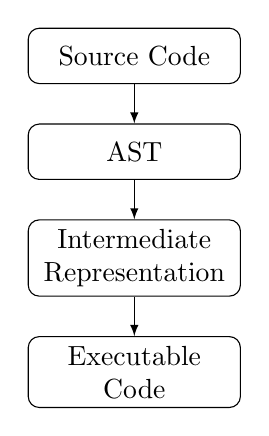
\begin{tikzpicture} 
    \node[block] (source) {Source Code}; 
    \node[block, below=0.5cm of source] (ast) {AST};
    \node[block, below=0.5cm of ast] (ir) {Intermediate Representation};
    \node[block, below=0.5cm of ir] (exe) {Executable Code};

    \draw[-latex] (source.south) -- node[above] {} (ast.north);
    \draw[-latex] (ast.south) -- node[above] {} (ir.north);
    \draw[-latex] (ir.south) -- node[above] {} (exe.north);
  \end{tikzpicture} 
  \caption{Traditional compiler pipeline (simplified)} 
  \label{fig:pipeline-static}
\end{figure}

In contrast, iterative compilation allows data to flow ``backwards'' through the
pipeline. Output from a stage can inform the action of a previous stage (on the
next compilation of the program).

\section{Evaluation} \label{sec:eval}

\subsection{Strategy}

\subsection{Comparison with Static Analysis} \label{ssec:compare}

\subsection{Possible Improvements and Further Work}

\section{Conclusion}

\ifCLASSOPTIONcaptionsoff
  \newpage
\fi

\printbibliography

\end{document}
